\documentclass{jsarticle}
\usepackage[margin = .7in]{geometry}
\usepackage[dvipdfmx]{graphicx}
\usepackage{listings}
\usepackage{amsmath}
\usepackage{bm}
\usepackage{ascmac}
\lstset{%
  language={python},
  basicstyle={\small},%
  identifierstyle={\small},%
  commentstyle={\small\itshape},%
  keywordstyle={\small\bfseries},%
  ndkeywordstyle={\small},%
  stringstyle={\small\ttfamily},
  frame={tb},
  breaklines=true,
  columns=[l]{fullflexible},%
  numbers=left,%
  xrightmargin=0zw,%
  xleftmargin=3zw,%
  numberstyle={\scriptsize},%
  stepnumber=1,
  numbersep=1zw,%
  lineskip=-0.5ex%
}

\begin{document}
\title{卒論テーマ候補 :ゆびすま2}
\author{池上 慧}
\maketitle

\section{ゲームの概要}
\subsection{ゆびすまとは}
「ゆびすま」とは2人以上で行われるゲームである。ここでは2人で行われるケースを想定する。プレイヤーは「攻め」と「守り」の役目を交互に行う。プレイヤーは毎回好きな本数の親指を上げる。「攻め」のプレイヤーは今回上がる親指の本数を予想し、その予想した数をコールしながら、自分でも好きな本数だけ親指を上げる。「守り」のプレイヤーも掛け声と同時に親指を好きな本数だけあげる。「攻め」がコールした数と実際にあげられた親指の総数が等しかったなら「攻め」の勝ちであり、そうでなければ「引き分け」である。引き分けたら役割を交代してどちらかが勝つまで続けるものとする。本来であれば勝てば腕を一本減らすことができ、先に二回勝利した方の勝ちというルールであるが、ここでは最初の2本vs2本の状況のみを想定する。

\subsection{ゲームの構造}
このゲームで勝敗を決するのは攻め手が決定する「宣言」と「指」との差である。この差で攻め手の行動を分類することができる。すなわち相手の上げる指の数が0本の時勝利する行動の組である$\left\{ (0,0), (1,1), (2,2)\right\}$をset1とし、相手の指の数が1本の時に勝利する行動の組である$\left\{ (1,0), (2,1), (3,2)\right\}$をset2、相手の指の数が2本の時に勝利する行動の組である$\left\{ (2,0), (3,1), (4,2)\right\}$をset3とする。これを用いてゲームの利得表は以下のように与えられる。
\begin{figure}[h]
    \centering
    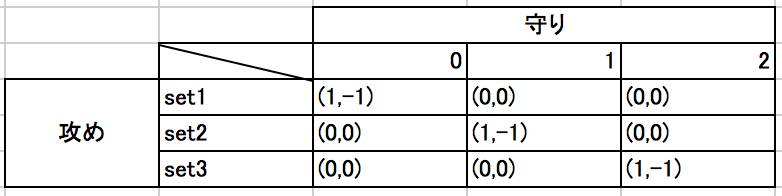
\includegraphics[width=10cm]{pmat.png}
    \caption{利得表}
\end{figure}
2人対称ゼロサムゲームとなる。これに対して混合戦略ナッシュ均衡は

\end{document}



































